%%%%%%%%%%%%%%%%%%%%%%%%%%%%%%%%%%%%%%%%%
% Beamer Presentation
% LaTeX Template
% Version 1.0 (10/11/12)
%
% This template has been downloaded from:
% http://www.LaTeXTemplates.com
%
% License:
% CC BY-NC-SA 3.0 (http://creativecommons.org/licenses/by-nc-sa/3.0/)
%
%%%%%%%%%%%%%%%%%%%%%%%%%%%%%%%%%%%%%%%%%

%----------------------------------------------------------------------------------------
%	PACKAGES AND THEMES
%----------------------------------------------------------------------------------------

\documentclass{beamer}

\mode<presentation> {

% The Beamer class comes with a number of default slide themes
% which change the colors and layouts of slides. Below this is a list
% of all the themes, uncomment each in turn to see what they look like.

%\usetheme{default}
%\usetheme{AnnArbor}
%\usetheme{Antibes}
%\usetheme{Bergen}
%\usetheme{Berkeley}
%\usetheme{Berlin}
%\usetheme{Boadilla}
%\usetheme{CambridgeUS}
%\usetheme{Copenhagen}
%\usetheme{Darmstadt}
%\usetheme{Dresden}
%\usetheme{Frankfurt}
%\usetheme{Goettingen}
%\usetheme{Hannover}
%\usetheme{Ilmenau}
%\usetheme{JuanLesPins}
%\usetheme{Luebeck}
\usetheme{Madrid}
%\usetheme{Malmoe}
%\usetheme{Marburg}
%\usetheme{Montpellier}
%\usetheme{PaloAlto}
%\usetheme{Pittsburgh}
%\usetheme{Rochester}
%\usetheme{Singapore}
%\usetheme{Szeged}
%\usetheme{Warsaw}

% As well as themes, the Beamer class has a number of color themes
% for any slide theme. Uncomment each of these in turn to see how it
% changes the colors of your current slide theme.

%\usecolortheme{albatross}
%\usecolortheme{beaver}
%\usecolortheme{beetle}
%\usecolortheme{crane}
%\usecolortheme{dolphin}
%\usecolortheme{dove}
%\usecolortheme{fly}
%\usecolortheme{lily}
%\usecolortheme{orchid}
%\usecolortheme{rose}
%\usecolortheme{seagull}
%\usecolortheme{seahorse}
%\usecolortheme{whale}
%\usecolortheme{wolverine}

%\setbeamertemplate{footline} % To remove the footer line in all slides uncomment this line
%\setbeamertemplate{footline}[page number] % To replace the footer line in all slides with a simple slide count uncomment this line

%\setbeamertemplate{navigation symbols}{} % To remove the navigation symbols from the bottom of all slides uncomment this line
}

\usepackage{graphicx} % Allows including images
\usepackage{booktabs} % Allows the use of \toprule, \midrule and \bottomrule in tables
\usepackage{tikz}
\usepackage{graphicx}
\graphicspath{ {images/} }
%----------------------------------------------------------------------------------------
%	TITLE PAGE
%----------------------------------------------------------------------------------------

\title[Short title]{C\'alculo de Congruencias} % The short title appears at the bottom of every slide, the full title is only on the title page

\author{Calcular todas las congruencias del reticulado\\ (\{1,2,3,6,12\}, mcm, mcd)}

\begin{document}

\begin{frame}
\titlepage % Print the title page as the first slide
\end{frame}


%----------------------------------------------------------------------------------------
%	PRESENTATION SLIDES
%----------------------------------------------------------------------------------------

%------------------------------------------------
\section{First Section}
%------------------------------------------------

\subsection{Subsection Example}

\begin{frame}
\frametitle{C\'alculo de Congruencias}
El reticulado (\{1,2,3,6,12\}, mcm, mcd) puede ser representado mediante el siguiente diagrama de Hasse.\\

\begin{center}
\begin{tikzpicture}
    \node (top) at (0,3) {$12$};
    \node (a) at (0,2) {$6$};
    \node (b) at (-1,1) {$2$};
    \node (c) at (1,1) {$3$};
    \node (min) at (0,0) {$1$};
    \draw (top) -- (a) -- (b) -- (min);
    \draw (a) -- (c) -- (min);

\end{tikzpicture}
\end{center}
\end{frame}

\begin{frame}

Asumiremos que se tiene la prueba del siguiente lemma (lemma de convexidad)
\begin{lemma}
Si $c \in L/ \theta $, entonces c es un subconjunto convexo de (L,s,i), es decir
    para cualesquiera $x,y,z \in L,$ si se da que $x,y \in c, $ y $x \leq z \leq y$, entonces $ z \in c $
\end{lemma}

\end{frame}

\begin{frame}
A continuaci\'on listaremos algunos teoremas que valen para todas las congruencias del reticulado que luego probaremos
\begin{theorem}

\[  6 \theta 3 =>  2 \theta 1 \]
\[  3 \theta 1 =>  2 \theta 6 \]
\[  2 \theta 6 =>  3 \theta 1 \]
\[  2 \theta 3 =>  1 \theta 2 \land 1\theta3 \land 6\theta2 \land 6\theta3 \]
\[  1 \theta 6 =>  1 \theta 2 \land 1\theta3 \land 6\theta2 \land 6\theta3 \]
\[  12 \theta 6 =>  6 \theta 3 \land  6\theta2 \]

\end{theorem}
\end{frame}

\begin{frame}
\frametitle{Congruencias Candidatas}
Por ser reticulado, sabemos que valen las congruencias triviales
\begin{center}


$\bigtriangledown$ 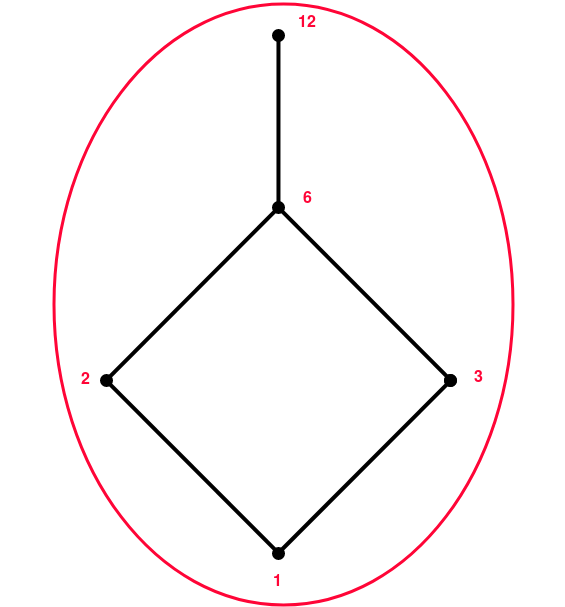
\includegraphics[height=5cm]{trivial_1}
$\bigtriangleup$ 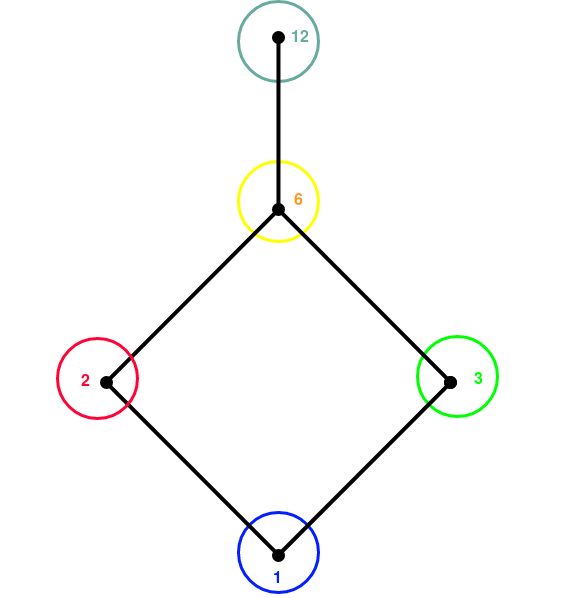
\includegraphics[height=5cm]{trivial_2}
\end{center}
\end{frame}
%------------------------------------------------

\begin{frame}
\frametitle{Congruencias Candidatas}
\begin{center}
1. 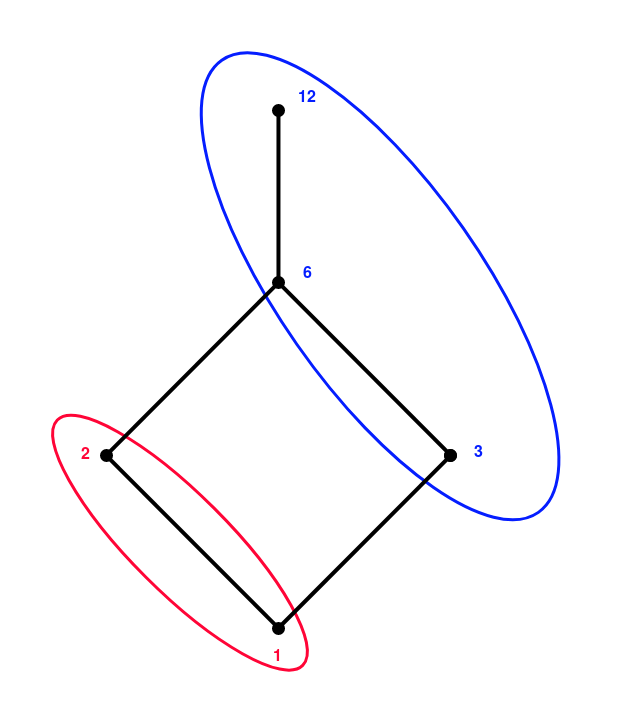
\includegraphics[height=5cm]{congruencia_1}
2. 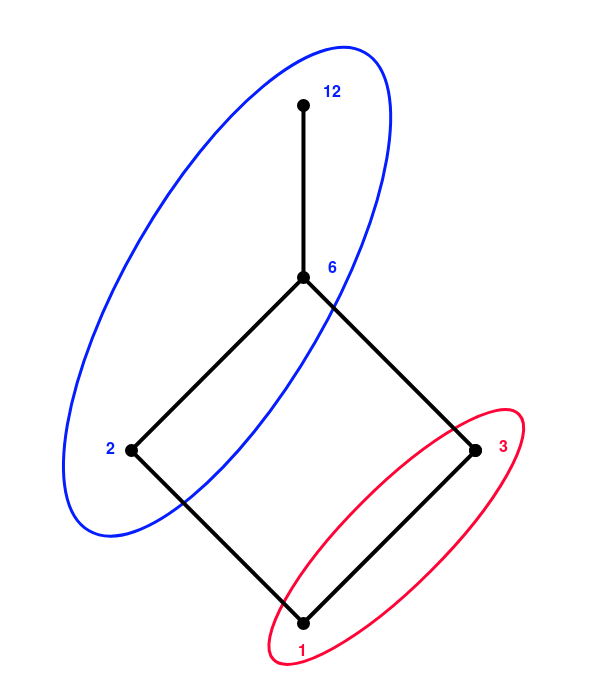
\includegraphics[height=5cm]{congruencia_2}
\end{center}
\end{frame}

%------------------------------------------------

\begin{frame}
\frametitle{Congruencias Candidatas}
\begin{center}
3. 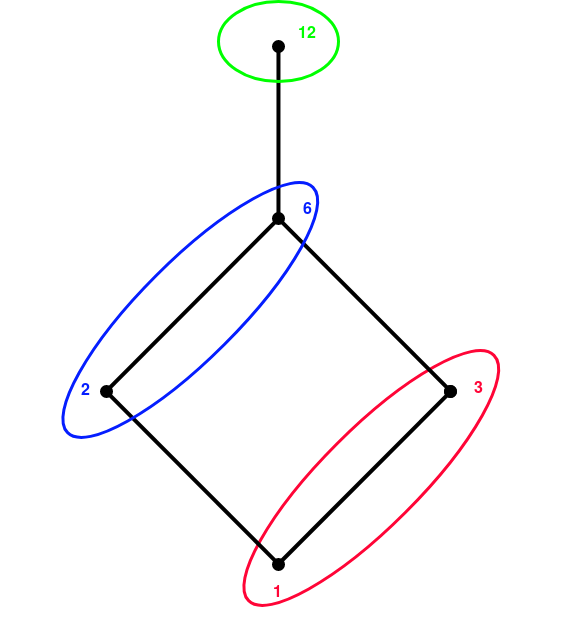
\includegraphics[height=5cm]{congruencia_3}
4. 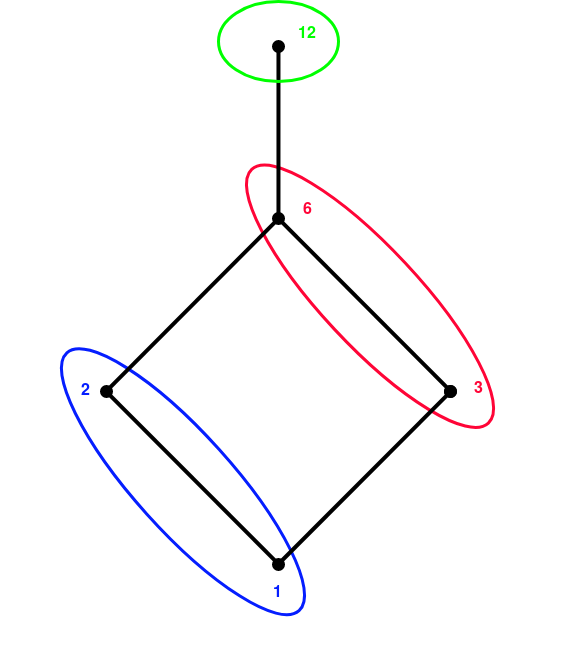
\includegraphics[height=5cm]{congruencia_4}
\end{center}
\end{frame}

%----------------------------------------------------------------------------------------
\begin{frame}
\frametitle{Congruencias Candidatas}
\begin{center}
5. 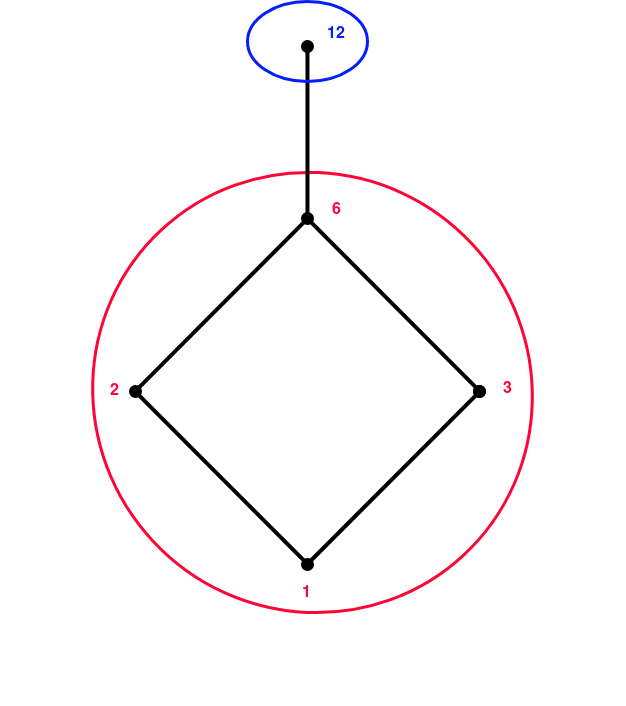
\includegraphics[height=5cm]{congruencia_5}
6. 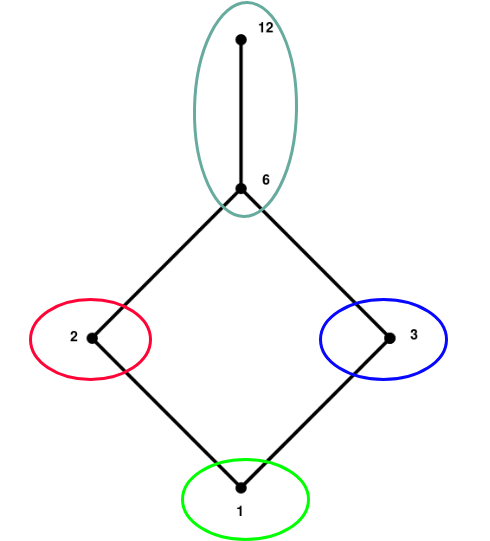
\includegraphics[height=5cm]{congruencia_6}
\end{center}
\end{frame}

%----------------------------------------------------------------------------------------
\begin{frame}
\frametitle{Congruencias. Caso $12/\theta=\{12\}.$}
Sea $\theta$ una congruencia sobre (\{1,2,3,6,12\},mcm,mcd) .\\

\noindent Ahora supongamos que $12/\theta=\{12\}.$\\
Analizaremos por casos todas las posibles congruencias\\
\textbf{Subcaso }$(6,1)$ $\in$ $\theta$ \\
\begin{itemize}
	\item     Si $(6,1)$ $\in$ $\theta$ entonces (por lema de convexidad)
    $\{6,3,2,1\} \subseteq 6/\theta$, y ya que $12/\theta=\{12\}$, entonces $6/\theta = \{6,3,2,1\}$ por lo tanto $\theta$ es la congruencia 5.\\
\end{itemize}
\end{frame}

\begin{frame}
\frametitle{Congruencias. Caso $12/\theta=\{12\}.$}
\textbf{Subcaso} (6,1) $\not \in \theta$
\begin{itemize}
\item Veamos el caso que $(2,1)$ $\in$ $\theta$ entonces (por lemita) $(3,6)$ $\in$
    $\theta$, por lo tanto $\theta$ es la congruencia 4.\\

\item Veamos el caso que $(3,1)$ $\in$ $\theta$ entonces (por lemita) $(2,6)$ $\in$
    $\theta$, por lo tanto $\theta$ es la congruencia 3.\\  

\end{itemize}
    
\end{frame}

\begin{frame}
\frametitle{Congruencias. Caso $12/\theta=\{12\}.$}
Nos queda analizar el caso en que\\
    $(2,3)$ $\in$ $\theta$, entonces (por lemita) $\{6,3,2,1\} \subseteq
    2/\theta$, ya que $12/\theta=\{12\}$, entonces $\{6,3,2,1\} = 2/\theta$.
    Pero esto implica que $(6,1)$ $\in$ $\theta$. Absurdo!\\
    Por lo tanto este caso no puede darse.
    Si no se da ninguno de los casos listados recien, entonces $a/\theta={a}$ para cada $a \in
    \{1,2,3,6,12\}$, por lo tanto $\theta$ es la congruencia $\bigtriangleup$ (la trivial).\\


\end{frame}

%----------------------------------------------------------------------------------------
\begin{frame}
\frametitle{Congruencias. Caso $12/\theta \not = \{12\}$}
Ahora veremos las congruencias donde $12/\theta \not = \{12\}$\\
\textbf{Subcaso $12/\theta = \{12,6\}$}
\begin{itemize}
\item Sabemos que $(2,1)$,$(3,1)$ $\notin$ $\theta$ (porque, por
    lemitas, eso implicaría que $(3,6)$ o $(2,6)$ $\in$ $\theta$, lo cual no puede
    ser porque supusimos que $12/\theta = \{12,6\}$). Entonces $\theta$ es la congruencia 6.\\
\end{itemize}    
\end{frame}
%----------------------------------------------------------------------------------------

\begin{frame}
\frametitle{Congruencias. Caso $12/\theta \not = \{12\}$}
\begin{itemize}

\item Si $3 \in 12/\theta$, por lema de convexitud, $6 \in 12/\theta$. Luego $(3,6)$ $\in$ $\theta$ implica (por lemita) $(2,1)$ $\in$ $\theta$.
\begin{itemize}
\item Luego, si $2 \notin 12/\theta$, entonces $\theta$ es la congruencia 1. 

\item Si $2 \in 12/\theta$ (por lemita), entonces $\theta$ es la congruencia $\bigtriangledown$ (la trivial total).\\
\end{itemize}
    
\item Si $2 \in 12/\theta$, por lema de convexidad, $6 \in 12/\theta$. Luego $(2,6)$ $\in$ $\theta$ implica (por lemita) $(3,1)$ $\in$ $\theta$. 
\begin{itemize}
\item Luego, si $3 \notin 12/\theta$, entonces $\theta$ es la congruencia 2.
\item Si $3 \in 12/\theta$ (por lemita), $\theta$ es la congruencia $\bigtriangledown$ (la trivial total).\\
\end{itemize}
\end{itemize}

\end{frame}

%----------------------------------------------------------------------------------------
\begin{frame}
\frametitle{Congruencias Caso $12/\theta \not = \{12\}$}
\begin{itemize}
\item     Si $1 \in 12/\theta$, por lema de convexidad, $12/\theta = \{12,6,3,2,1\}$, por lo tanto $\theta$ es la congruencia $\bigtriangledown$ (trivial total).\\
\end{itemize}
Con esto ya cubrimos todas las posibles congruencias $\theta$.
\end{frame}

%----------------------------------------------------------------------------------------

\begin{frame}
\frametitle{Prueba Lemitas}
Veamos ahora los lemas que planteamos sobre este reticulado valen:\\
\begin{enumerate}
\item[(a)] $6\theta 3$ $\Rightarrow$ $2\theta 1$\\
       $6\theta 3$ $\Rightarrow$ $6i2\theta 3i2$ $\Rightarrow$ $2\theta 1$\\

\item[(b)] $3\theta 1$ $\Rightarrow$ $2\theta 6$\\
       $3\theta 1$ $\Rightarrow$ $3s2\theta 1s2$ $\Rightarrow$ $6\theta 2$ $\Rightarrow$ $2\theta 6$\\
       
\item[(c)] $2\theta 6$ $\Rightarrow$ $3\theta 1$\\
       $2\theta 6$ $\Rightarrow$ $2i3\theta 6i3$ $\Rightarrow$ $1\theta 3$ $\Rightarrow$ $3\theta 1$\\

\end{enumerate}
\end{frame}
%----------------------------------------------------------------------------------------

\begin{frame}
\frametitle{Prueba Lemitas}
\begin{enumerate}
\item[(d)] $2\theta 3$ $\Rightarrow$ $1\theta 2$ y $1\theta 3$ y $6\theta 2$
       y $6\theta 3$\\
       $2\theta 3$ $\Rightarrow$ $3\theta 3$ y $2\theta 3$ $\Rightarrow$
       $3s2\theta 3s3$ y $3i2\theta 3i3$\\ 
       $\Rightarrow$ $6\theta 3$ y $1\theta 3$\\
       Por (a) si $6\theta 3$ $\Rightarrow$ $2\theta 1$;Por (b) si $3\theta 1$
       $\Rightarrow$ $2\theta 6$\\
       Por lo tanto si $2\theta 3$ $\Rightarrow$ $1\theta 2$ y $1\theta 3$ y $6\theta 2$
       y $6\theta 3$\\

\item[(e)] $1\theta 6$ $\Rightarrow$ $1\theta 2$ y $1\theta 3$ y $6\theta 2$
       y $6\theta 3$\\
       $1\theta 6$ $\Rightarrow$ $1s2\theta 6s2$ $\Rightarrow$ $2\theta 6$\\
       $1\theta 6$ $\Rightarrow$ $1s3\theta 6s3$ $\Rightarrow$ $3\theta 6$\\
       Por (a) si $6\theta 3$ $\Rightarrow$ $2\theta 1$.\\
       Si $6\theta 2$ y $6\theta 3$ $\Rightarrow$ $2\theta 3$
       $\Rightarrow$ $1\theta 3$.
\end{enumerate}
\end{frame}

\begin{frame}
\frametitle{Conclusi\'on}
Con esto hemos probado cuales son todas las congruencias del reticulado (\{1,2,3,6,12\},mcm,mcd). 
\end{frame}
\end{document} 
